% ============================================================
% Chapter 22: Hilbert's Problem 21 — The Monodromy Theorem
% ============================================================

\chapter{The Monodromy Theorem}

\begin{solvedbox}
\textbf{Solved.} Hilbert's twenty-first problem asked for a proof of the \emph{monodromy theorem}---that a function analytically continued along paths in a simply connected domain always returns to its original value---and its extension to more general situations. The theorem was proved in the late nineteenth century by Poincar\'e and others, and it has since become a standard result in complex analysis. Its modern formulation, cast in the language of covering spaces and the fundamental group, is a standard part of the graduate curriculum and a bridge between analysis and topology.
\end{solvedbox}

% ------------------------------------------------------------
\section{Historical Context}
% ------------------------------------------------------------

In the early nineteenth century, mathematicians confronted a peculiar phenomenon. Certain functions, perfectly well-defined locally, seemed to ``grow'' new branches when examined globally. The square root function $\sqrt{z}$, the logarithm $\log z$, and the inverse trigonometric functions all shared this property: they could not be defined as single-valued functions on the entire complex plane without encountering a discontinuity.

This was not a defect of the functions but a reflection of the topology of the complex plane with points removed. The question was how to make sense of it rigorously.

\subsection{Riemann and Multivalued Functions}

Bernhard Riemann (1826--1866) gave the decisive insight. In his 1851 doctoral dissertation, \emph{Grundlagen f\"ur eine allgemeine Theorie der Funktionen einer ver\"anderlichen komplexen Gr\"osse} (``Foundations for a General Theory of Functions of a Complex Variable''), Riemann introduced what we now call \textbf{Riemann surfaces}: sheets of the complex plane glued together along branch cuts, on which a multivalued function becomes single-valued.

Consider the function $w = \sqrt{z}$. If we start at $z = 1$ with $\sqrt{1} = 1$ and continuously deform $z$ along a circle $|z| = 1$ back to $z = 1$, the value of $\sqrt{z}$ does \emph{not} return to $1$; it returns to $-1$. We must traverse the circle \emph{twice} to return to the original value. Riemann's idea was to replace the single complex plane with a two-sheeted surface---two copies of $\mathbb{C}$ glued along a ray from the origin---on which $\sqrt{z}$ becomes a genuine single-valued function.

This was significant. Rather than viewing multivaluedness as a problem to be avoided, Riemann embraced it as a feature of the underlying geometry. The function was not poorly defined; the domain was too simple.

\subsection{Analytic Continuation}

Riemann's work was built on the earlier notion of \textbf{analytic continuation}. The idea is elementary: if two analytic functions agree on a region where they overlap, they are ``the same function'' continued to a larger domain.

\begin{definition}[Analytic continuation]
Let $f_1$ be analytic in an open set $\Omega_1$ and $f_2$ analytic in an open set $\Omega_2$, with $\Omega_1 \cap \Omega_2 \neq \varnothing$. We say $f_2$ is an \textbf{analytic continuation} of $f_1$ if $f_1(z) = f_2(z)$ for all $z \in \Omega_1 \cap \Omega_2$.
\end{definition}

The power of analytic continuation rests on the \textbf{identity theorem}: if two analytic functions agree on a set with an accumulation point in their common domain, they agree everywhere. This means that if we can continue a function along two different paths to the same endpoint, the results will agree---\emph{provided the paths are homotopic} (continuously deformable into each other).

But what if the paths are \emph{not} homotopic? What if the domain has holes? Then analytic continuation along different paths can yield different values. This phenomenon is called \textbf{monodromy}.

\subsection{The Monodromy Group}

If we analytically continue a function along every closed loop in a domain $\Omega$, we obtain a permutation of the branches of the function. The collection of all such permutations, for all closed loops, forms a group---the \textbf{monodromy group}.

Poincar\'e formalized this idea in the 1880s and 1890s, in the context of his work on Fuchsian and Kleinian groups. Fuchsian groups are discrete subgroups of $\mathrm{PSL}(2, \mathbb{R})$ acting on the upper half-plane, and they arise as monodromy groups of second-order linear ODEs with regular singular points. Kleinian groups are their analogues for the Riemann sphere. Poincar\'e showed that the monodromy group encodes significant information about the global behavior of analytic functions and the geometry of the surfaces on which they live.

Hilbert, in his 1900 address, saw the monodromy theorem as a problem that deserved a rigorous and general treatment. The naive statement---that continuation along closed loops returns to the starting value---is true only in simply connected domains. The general question, for multiply connected domains, is exactly the question of the fundamental group and its action on the space of analytic continuations.

% ------------------------------------------------------------
\section{The Problem}
% ------------------------------------------------------------

\begin{problem_statement}[Hilbert's Twenty-First Problem]
Prove the monodromy theorem: that a function element, analytically continued along all possible paths in a simply connected domain, returns to its original value at the starting point. Extend this result to more general domains, where the behavior of continuation is governed by the topology of the domain.
\end{problem_statement}

Let us unpack the key concepts.

\subsection{What Is Analytic Continuation?}

A \textbf{function element} is a pair $(f, \Omega)$ where $\Omega$ is an open connected set and $f$ is analytic on $\Omega$. Two function elements $(f_1, \Omega_1)$ and $(f_2, \Omega_2)$ are \emph{equivalent} if they agree on their overlap: $f_1 = f_2$ on $\Omega_1 \cap \Omega_2 \neq \varnothing$.

A \textbf{chain of function elements} from $(f_0, \Omega_0)$ to $(f_n, \Omega_n)$ is a sequence of function elements $(f_0, \Omega_0), (f_1, \Omega_1), \ldots, (f_n, \Omega_n)$ such that each consecutive pair agrees on their overlap. This chain defines the analytic continuation of $f_0$ along a path in the union of the $\Omega_k$.

The fundamental question is: does the result depend on the path chosen?

\subsection{What Is Monodromy?}

Given a function element $(f, \Omega)$ and a closed loop $\gamma$ in $\Omega$ based at a point $z_0$, we can analytically continue $f$ along $\gamma$. If the continuation returns to the same branch---that is, the continued function agrees with $f$ near $z_0$---then $\gamma$ is said to be \emph{transparent} to $f$. If the continuation lands on a different branch, the loop $\gamma$ has \emph{monodromy} for $f$.

\begin{figure}[htbp]
\centering
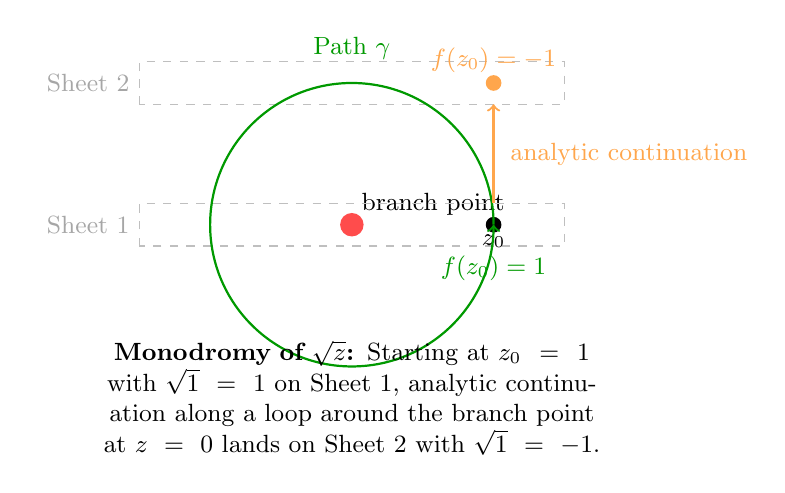
\begin{tikzpicture}[
    scale=0.9,
    font=\small,
    path/.style={->, thick, color=blue!70},
    branch/.style={circle, fill=red!70, inner sep=3pt},
    point/.style={circle, fill=black, inner sep=2pt},
    sheet/.style={draw, dashed, color=gray!50}
]

% Branch point at origin
\node[branch] at (0,0) {};
\node[above right] at (0,0) {branch point};

% First sheet (bottom)
\draw[sheet] (-3,-0.3) rectangle (3,0.3);
\node[left, color=gray!70] at (-3,0) {Sheet 1};

% Second sheet (top)
\draw[sheet] (-3,1.7) rectangle (3,2.3);
\node[left, color=gray!70] at (-3,2) {Sheet 2};

% Base point
\node[point] at (2,0) {};
\node[below] at (2,0) {$z_0$};

% Path going around branch point (on Sheet 1)
\draw[path, color=green!60!black] (2,0) arc (0:360:2);
\node[above, color=green!60!black] at (0,2.2) {Path $\gamma$};

% Arrow showing continuation
\draw[->, thick, color=orange!70] (2,0.3) -- (2,1.7);
\node[right, color=orange!70] at (2.1,1) {analytic continuation};

% Result on Sheet 2
\node[point, color=orange!70] at (2,2) {};
\node[above, color=orange!70] at (2,2) {$f(z_0) = -1$};

% Start value
\node[below, color=green!60!black] at (2,-0.3) {$f(z_0) = 1$};

% Labels
\node[below, align=center, text width=8cm] at (0, -1.5) {
    \textbf{Monodromy of $\sqrt{z}$:} Starting at $z_0 = 1$ with $\sqrt{1} = 1$ on Sheet 1, analytic continuation along a loop around the branch point at $z = 0$ lands on Sheet 2 with $\sqrt{1} = -1$.
};

\end{tikzpicture}
\caption{Analytic continuation of $w = \sqrt{z}$ around the branch point at $z = 0$. The function starts on Sheet 1 with $\sqrt{1} = 1$, but after traversing a loop around the branch point, it lands on Sheet 2 with $\sqrt{1} = -1$. This demonstrates nontrivial monodromy---the function does not return to its original value.}
\label{fig:monodromy}
\end{figure}

For a simply connected domain, every closed loop is contractible to a point, and the monodromy theorem guarantees that every loop is transparent. But for a domain with holes, non-contractible loops can produce genuine monodromy.

% ------------------------------------------------------------
\section{Key Developments}
% ------------------------------------------------------------

\subsection{The Monodromy Theorem for Simply Connected Domains}

The monodromy theorem is one of the most important results in complex analysis.

\begin{theorem}[Monodromy Theorem]
\label{thm:monodromy}
Let $\Omega$ be a simply connected open set in $\mathbb{C}$, and let $\gamma \colon [0,1] \to \Omega$ be a closed loop based at $z_0 \in \Omega$. If $(f_0, U_0)$ is a function element at $z_0$ that can be analytically continued along every path in $\Omega$, then continuation along $\gamma$ returns to the original function element $f_0$.
\end{theorem}

\begin{proof}
Since $\Omega$ is simply connected, the loop $\gamma$ is homotopic to the constant loop at $z_0$ within $\Omega$. That is, there exists a continuous map $H \colon [0,1] \times [0,1] \to \Omega$ with $H(0,t) = H(1,t) = z_0$ for all $t$, and $H(s,0) = \gamma(s)$ for all $s$.

For each $t$, the path $\gamma_t(s) = H(s,t)$ is a closed loop based at $z_0$. Let $f_t$ denote the result of analytically continuing $f_0$ along $\gamma_t$. We need to show that $f_1 = f_0$.

The function $F(s,t) = f_t(s)$---the value obtained by continuing along $\gamma_t$ to the point $H(s,t)$---is jointly continuous in $(s,t)$ (by the continuity of analytic continuation with respect to deformation of paths) and analytic in $z = H(s,t)$ for each fixed $t$. The key point is that analytic continuation depends continuously on the path, and the space of analytic function elements at $z_0$ is \emph{discrete} (by the identity theorem, two function elements at $z_0$ are either equal or different in a neighborhood of $z_0$).

Since $t \mapsto f_t$ is continuous and the target is discrete, it must be constant. Therefore $f_1 = f_0$.
\end{proof}

The key insight is that analytic continuation is a \emph{local-to-global} principle: the local uniqueness of analytic functions (the identity theorem) forces global consistency when the domain has no holes.

\subsection{Covering Spaces and the Fundamental Group}

The monodromy theorem admits a notable reformulation in the language of algebraic topology, which became standard in the twentieth century.

\begin{definition}[Fundamental group]
Let $X$ be a topological space and $x_0 \in X$ a base point. The \textbf{fundamental group} $\pi_1(X, x_0)$ is the group of homotopy classes of closed loops in $X$ based at $x_0$, with the operation given by concatenation of loops.
\end{definition}

\begin{definition}[Covering space]
A \textbf{covering space} of $X$ is a space $\tilde{X}$ together with a continuous surjection $p \colon \tilde{X} \to X$ such that every $x \in X$ has an open neighborhood $U$ with the property that $p^{-1}(U)$ is a disjoint union of open sets each mapped homeomorphically onto $U$ by $p$.
\end{definition}

The connection to monodromy is this: given a function element $(f_0, U_0)$ that can be analytically continued along all paths in $\Omega$, the \textbf{Riemann surface} of the function---the space of all function elements obtained by analytic continuation from $f_0$---is a covering space of $\Omega$.

\begin{theorem}[Monodromy Theorem, Topological Form]
\label{thm:monodromy-topological}
Let $p \colon \tilde{\Omega} \to \Omega$ be a covering space with $\Omega$ simply connected. Then for any base point $z_0 \in \Omega$, every closed loop in $\Omega$ lifts to a closed loop in $\tilde{\Omega}$. Equivalently, the monodromy action of $\pi_1(\Omega, z_0)$ on the fiber $p^{-1}(z_0)$ is trivial.
\end{theorem}

\begin{proof}
Since $\Omega$ is simply connected, $\pi_1(\Omega, z_0) = \{e\}$ is the trivial group. The monodromy representation $\rho \colon \pi_1(\Omega, z_0) \to \mathrm{Sym}(p^{-1}(z_0))$ therefore maps every element to the identity permutation. Every loop lifts to a closed loop.
\end{proof}

This is the topological heart of the matter. The monodromy theorem is not really a theorem about complex analysis---it is a theorem about the topology of simply connected spaces.

\subsection{Multiply Connected Domains and Monodromy Representations}

When $\Omega$ is \emph{not} simply connected, the fundamental group is nontrivial, and analytic continuation can produce genuine monodromy. The monodromy group is then a \emph{representation} of the fundamental group.

\begin{definition}[Monodromy representation]
Let $\Omega$ be a domain and $(f_0, U_0)$ a function element that can be analytically continued along all paths in $\Omega$. The \textbf{monodromy representation} is the group homomorphism
\[
    \rho \colon \pi_1(\Omega, z_0) \to \mathrm{Sym}(p^{-1}(z_0))
\]
that sends each homotopy class $[\gamma]$ to the permutation of the fiber induced by continuation along $\gamma$.
\end{definition}

The monodromy group is the image $\rho(\pi_1(\Omega, z_0))$, a subgroup of the symmetric group on the fiber.

\begin{example}
Consider $f(z) = \sqrt{z(z-1)}$ on $\Omega = \mathbb{C} \setminus \{0, 1\}$. The domain $\Omega$ is multiply connected, with $\pi_1(\Omega) \cong F_2$, the free group on two generators. The monodromy group of $\sqrt{z(z-1)}$ is $\mathbb{Z}/2\mathbb{Z}$, generated by the permutation that swaps the two branches.
\end{example}

\subsection{Connection to Riemann Surfaces}

The Riemann surface of a multivalued function is precisely the covering space whose monodromy group governs the branching behavior. For example:

\begin{itemize}
    \item The Riemann surface of $\sqrt{z}$ is a two-sheeted cover of $\mathbb{C} \setminus \{0\}$, with monodromy group $\mathbb{Z}/2\mathbb{Z}$.
    \item The Riemann surface of $\log z$ is an infinite-sheeted cover of $\mathbb{C} \setminus \{0\}$, with monodromy group $\mathbb{Z}$.
    \item The Riemann surface of $\sqrt[3]{z(z-1)}$ is a three-sheeted cover of $\mathbb{C} \setminus \{0, 1\}$, with monodromy group $\mathbb{Z}/3\mathbb{Z}$.
\end{itemize}

In general, a function with $n$ branches has a monodromy group that is a subgroup of $S_n$ (the symmetric group on $n$ letters). The structure of the monodromy group---its orbits, its fixed points, its transitivity---tells us about the geometry of the Riemann surface and the algebraic properties of the function.

\subsection{Historical Development and Modern Formulation}

The monodromy theorem was proved in various forms by Poincar\'e (1880s--1890s), and its connection to covering spaces was clarified by the development of algebraic topology in the early twentieth century. The modern formulation, using the language of the fundamental group and covering spaces, was fully articulated by Heinz Hopf and others in the 1920s and 1930s.

Lars Ahlfors, in his standard textbook \emph{Complex Analysis} (1953), presented the monodromy theorem as one of the central results of the subject, emphasizing its role as a bridge between local and global analysis. The theorem has since become standard material in any graduate course in complex analysis.

\subsection{Applications and Extensions}

The monodromy theorem has applications throughout mathematics:

\begin{itemize}
    \item \textbf{Hypergeometric functions:} The classical hypergeometric equation $z(1-z)w'' + [c - (a+b+1)z]w' - abw = 0$ has solutions with monodromy groups that are important in number theory and representation theory.
    \item \textbf{Algebraic geometry:} The monodromy theorem underlies the theory of algebraic de Rham cohomology and the comparison theorem between de Rham and Betti cohomology. The monodromy of a family of algebraic varieties is a key invariant in mirror symmetry and the theory of motives.
    \item \textbf{Differential equations:} The monodromy data of a linear ODE with regular singular points determines the equation up to isomorphism (the Riemann--Hilbert correspondence).
\end{itemize}

% ------------------------------------------------------------
\section{Current Status: Solved}
% ------------------------------------------------------------

\begin{solvedbox}
The monodromy theorem is \textbf{fully solved} in its classical form. The theorem for simply connected domains follows from basic topology (the triviality of the fundamental group), and the general theory of monodromy representations is a standard part of modern complex analysis and algebraic topology. The theorem has been extended in many directions: to several complex variables, to algebraic geometry (via the Riemann--Hilbert correspondence), and to the theory of perverse sheaves. The original problem posed by Hilbert has been comprehensively answered.
\end{solvedbox}

% ------------------------------------------------------------
\section*{Common Questions}
% ------------------------------------------------------------

\begin{description}[font=\bfseries, leftmargin=2em, style=nextline]

\item[Q: What is monodromy in everyday language?]\hfill\\
Imagine walking around a pillar while holding a rope tied to a fixed point. If the pillar is there, you cannot shrink your path; when you return, the rope is wrapped differently. Monodromy is the same phenomenon for functions: if the domain has ``holes'' (branch points), walking a loop around them can return the function to a different branch than the one you started with.

\item[Q: How does analytic continuation give rise to monodromy?]\hfill\\
Analytic continuation extends a function along a path by overlapping disks. If two paths from $A$ to $B$ are homotopic (can be deformed into each other), the results match. But if the domain is not simply connected, non-homotopic paths can land on different branches---this path-dependence is monodromy, and it measures the failure of the function to be single-valued.

\item[Q: What is the Riemann--Hilbert correspondence?]\hfill\\
It states that a linear ODE with regular singular points is completely determined by its monodromy data (the group of permutations of solutions under analytic continuation around the singularities). Conversely, any representation of the fundamental group can be realized as the monodromy of some ODE. This bridges differential equations, topology, and representation theory.

\item[Q: Why does simply connected guarantee ``no monodromy''?]\hfill\\
In a simply connected domain every loop is contractible to a point. Analytic continuation along a contractible loop returns to the starting branch because the identity theorem forces local agreement throughout the deformation. The fundamental group is trivial, so the monodromy representation has nowhere to be nontrivial.

\item[Q: What is the monodromy group of $\sqrt{z}$?]\hfill\\
It is $\mathbb{Z}/2\mathbb{Z}$. Looping once around $0$ swaps the two branches ($\sqrt{z} \mapsto -\sqrt{z}$); looping twice returns to the original. The group has exactly two elements: identity and the swap.

\item[Q: How does monodromy relate to Riemann surfaces?]\hfill\\
The Riemann surface of a multivalued function is precisely the covering space on which the function becomes single-valued. The monodromy group is the deck transformation group of this covering---the permutations of sheets induced by loops in the base. The more complicated the monodromy, the more sheets the Riemann surface needs.

\end{description}

% ------------------------------------------------------------
\section*{Exercises}
% ------------------------------------------------------------

\begin{enumerate}

    \item \textbf{Analytic continuation of $\log z$ around the origin.}
    \begin{enumerate}
        \item Let $f_0(z) = \log z$ with the principal branch ($-\pi < \operatorname{Arg} z \leq \pi$) defined on $\mathbb{C} \setminus (-\infty, 0]$. Analytically continue $f_0$ along the counterclockwise circle $\gamma(t) = e^{2\pi i t}$ for $t \in [0, 1]$. What value does the continued function take at $z = 1$ when $t = 1$?
        \item Continue the function along the circle $n$ times (i.e., $\gamma_n(t) = e^{2\pi i n t}$). What is the resulting value at $z = 1$?
        \item Describe the monodromy group of $\log z$ on $\mathbb{C} \setminus \{0\}$. What group is it isomorphic to?
    \end{enumerate}

    \item \textbf{Monodromy of $\sqrt{z^2 - 1}$.}
    Consider $f(z) = \sqrt{(z-1)(z+1)}$ on $\Omega = \mathbb{C} \setminus \{-1, 1\}$.
    \begin{enumerate}
        \item Identify two generators $\alpha, \beta$ of $\pi_1(\Omega, z_0)$ where $z_0 = 2i$ (one loop encircling $z = 1$, the other encircling $z = -1$). Describe these loops geometrically.
        \item Compute the monodromy of $f$ along $\alpha$ and $\beta$. What permutations of the two sheets do they induce?
        \item What is the monodromy group? Is it $\mathbb{Z}/2\mathbb{Z}$, $\mathbb{Z}/2\mathbb{Z} \times \mathbb{Z}/2\mathbb{Z}$, or something else?
        \item Compute the monodromy along the loop $\alpha\beta\alpha\beta^{-1}$ (the commutator). What do you observe?
    \end{enumerate}

    \item \textbf{The monodromy theorem for simply connected domains.}
    \begin{enumerate}
        \item State the monodromy theorem precisely, including all hypotheses.
        \item Explain why the theorem fails on $\mathbb{C} \setminus \{0\}$. Give an explicit example.
        \item Explain why the theorem holds on the slit plane $\mathbb{C} \setminus (-\infty, 0]$. Is this domain simply connected?
    \end{enumerate}

    \item \textbf{Riemann surfaces and covering spaces.}
    \begin{enumerate}
        \item Construct the Riemann surface of $w = \sqrt{z}$ explicitly. How many sheets does it have? Describe the branching behavior.
        \item Construct the Riemann surface of $w = \sqrt[3]{z}$. How many sheets? What is the monodromy group?
        \item Explain why the Riemann surface of $w = \sqrt{z(z-1)(z-2)}$ is a two-sheeted cover of $\mathbb{C} \setminus \{0, 1, 2\}$, and determine the monodromy representation.
    \end{enumerate}

    \item \textbf{The identity theorem and path dependence.}
    \begin{enumerate}
        \item State the identity theorem for analytic functions.
        \item Use the identity theorem to explain why two analytic continuations of the same function element along \emph{homotopic} paths must agree.
        \item Give an example of two paths in $\mathbb{C} \setminus \{0\}$ that are \emph{not} homotopic and along which the analytic continuation of $\sqrt{z}$ yields different values.
    \end{enumerate}

    \item[$\star$] \textbf{Monodromy of the hypergeometric function.}
    The hypergeometric equation
    \[
        z(1-z)w'' + [c - (a+b+1)z]w' - abw = 0
    \]
    has three regular singular points at $z = 0, 1, \infty$.
    \begin{enumerate}
        \item Explain why the monodromy group of a solution of the hypergeometric equation is a subgroup of $\mathrm{SL}(2, \mathbb{C})$ (acting on the two-dimensional space of solutions).
        \item For the special case $a = b = 1/2$, $c = 1$, the hypergeometric function reduces to $F(1/2, 1/2; 1; z) = \frac{2}{\pi} K(z)$, where $K$ is the complete elliptic integral of the first kind. Describe the monodromy of $K(z)$ and explain why it has period $2$ (up to a modular transformation) when $z$ is continued around $z = 1$.
        \item (Research question) The monodromy group of the hypergeometric equation is related to triangle groups in $\mathrm{PSL}(2, \mathbb{R})$. Look up the Schwarz triangle function and explain how it connects monodromy to hyperbolic geometry.
    \end{enumerate}

\end{enumerate}
